\chapter{设计}\label{chap:design}

\section{TileLink一致性协议}

\begin{figure}[H] %H为当前位置,!htb为忽略美学标准,htbp为浮动图形
\centering %图片居中
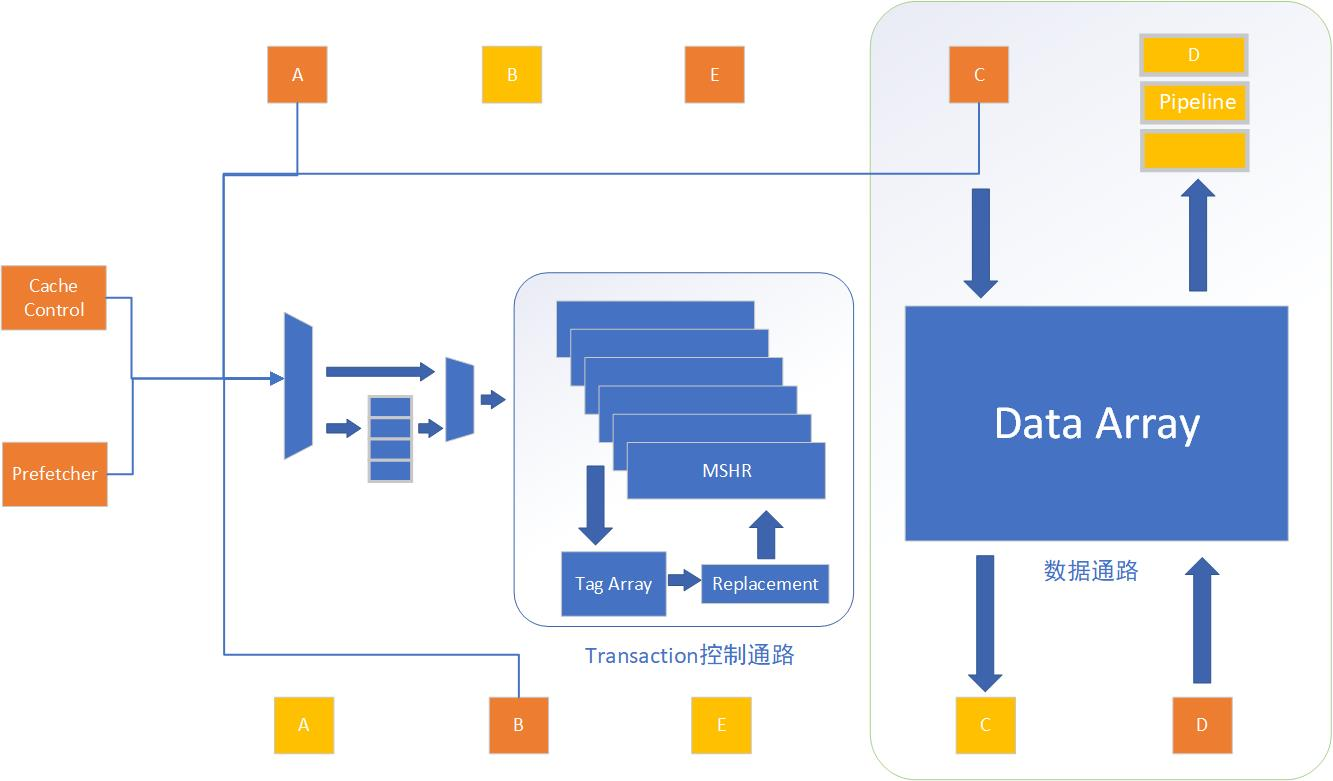
\includegraphics[width=\textwidth]{Img/BlockInclusiveCache.jpg} %插入图片,[]中设置图片大小,{}中是图片文件名
\caption{BlockInclusiveCache} %最终文档中希望显示的图片标题
\label{BlockInclusiveCache} %用于文内引用的标签
\end{figure}

\begin{figure}[H] %H为当前位置,!htb为忽略美学标准,htbp为浮动图形
\centering %图片居中
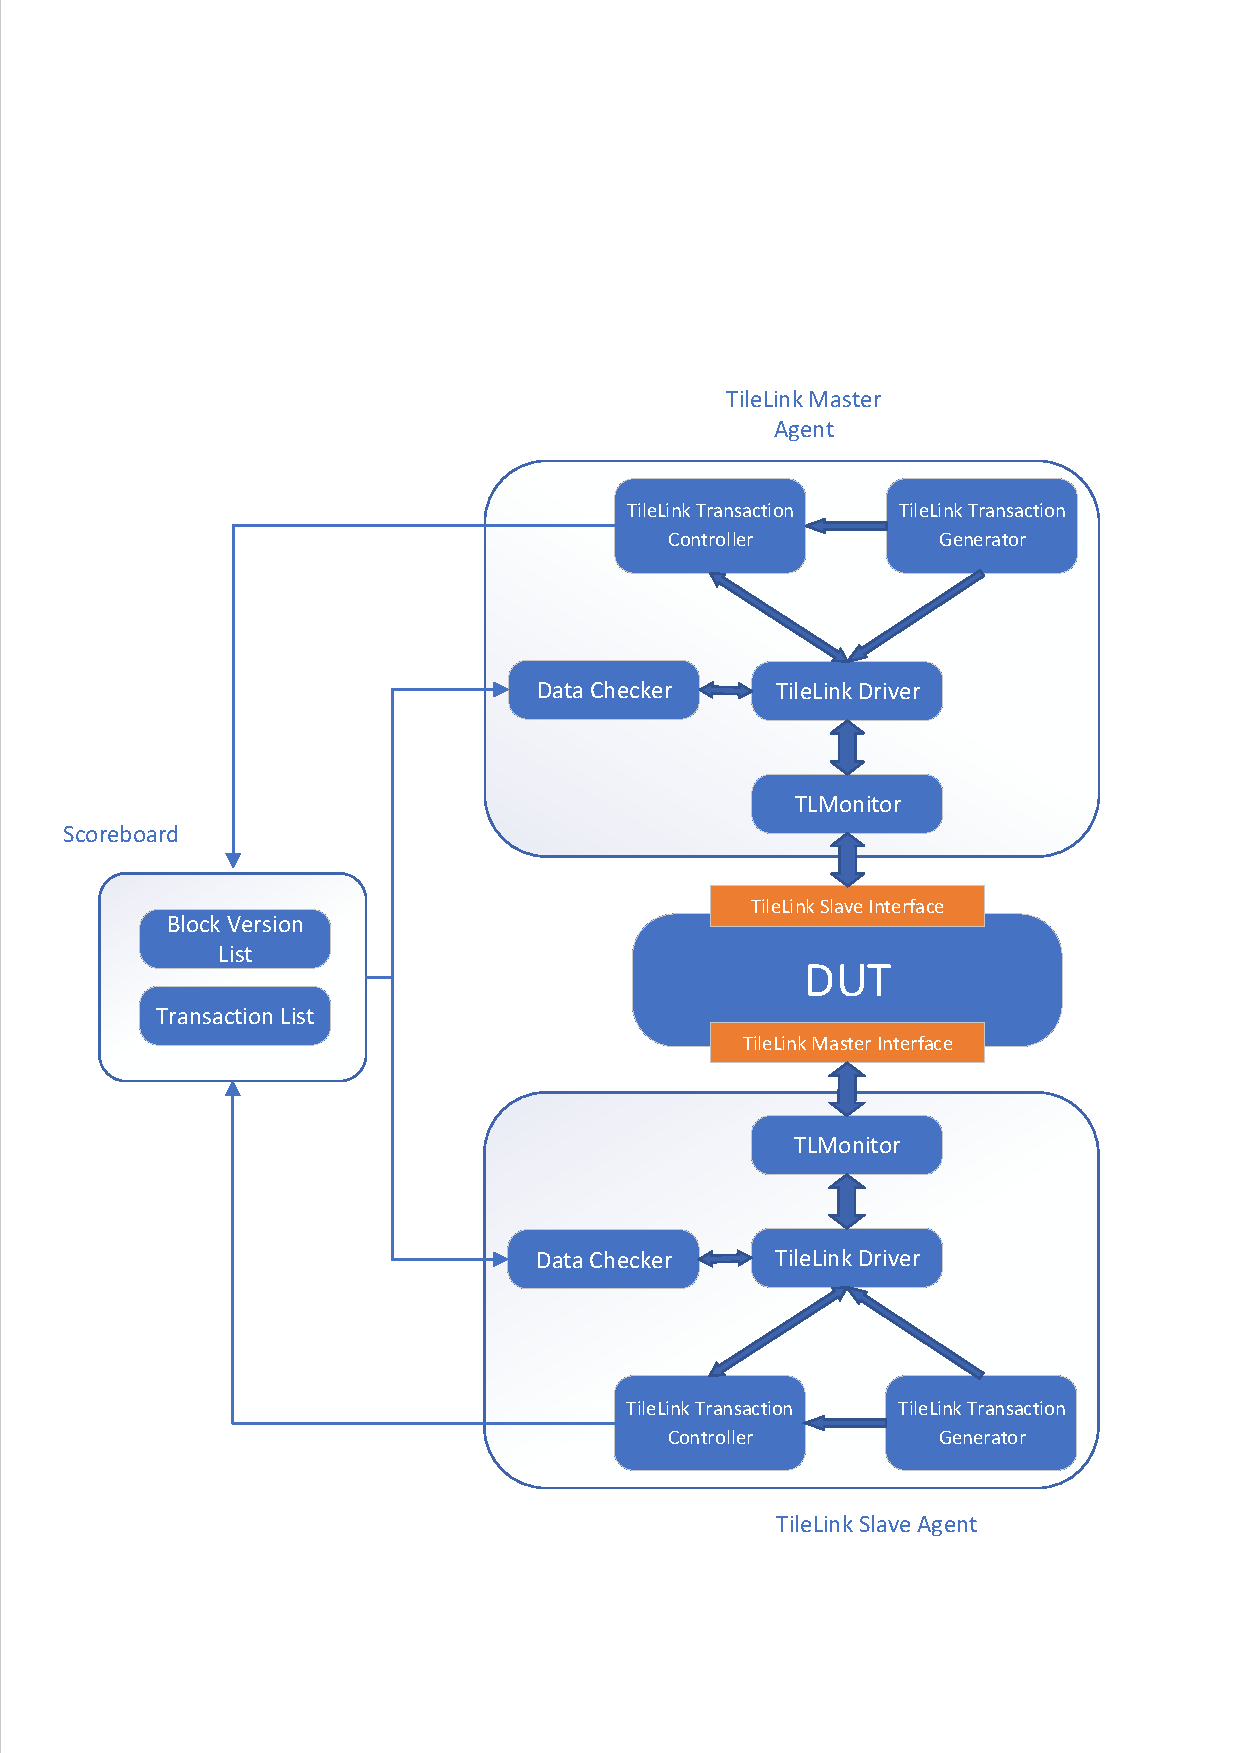
\includegraphics[width=\textwidth]{Img/BlockInclusiveCacheTest.pdf} %插入图片,[]中设置图片大小,{}中是图片文件名
\caption{BlockInclusiveCacheTest} %最终文档中希望显示的图片标题
\label{BlockInclusiveCacheTest} %用于文内引用的标签
\end{figure}
